% $Id: introduction.tex 34630 2013-04-29 22:53:51Z roldeman $

\section{The Level 1 Trigger Upgrade}
\label{sec:triggerupgrade}

With the upgrading of the LHC to $\sqrt{s}=13$ to $14$ TeV in 2015 the demands on the trigger are going to be greatly increased, particularly with the instantaneous luminosity increase \cite{TriggerTDR_Tapper:2013yva}. The calculations for triggering on the calorimeters are carried out with a Global Calorimeter Trigger (GCT). The ECAL and HCAL components are split into a $56\times 72$ grid of towers (TT) in $\eta$ and $\phi$ (the azimuthal angle), with each tower covering the area of $5\times5$ ECAL crystals. The GCT in the previous run had limited resources so the towers were grouped into $4\times4$ blocks, known as RCT regions, by the Regional Calorimeter Trigger. This is visually represented in Fig.~\ref{fig:trigger_calorimeter}.
\begin{figure}
	\begin{center}
		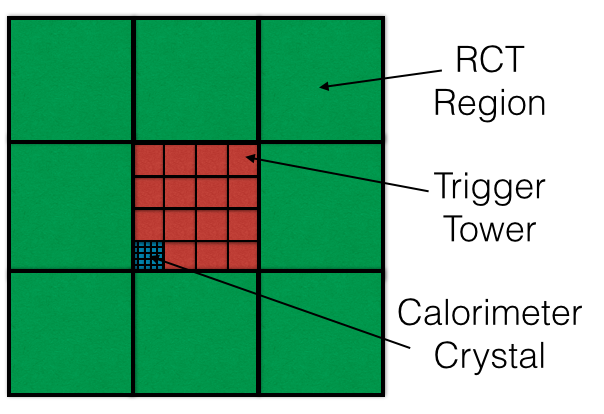
\includegraphics[width=0.4\linewidth]{trigger_calorimeter}
	\end{center}
	\caption{The various calorimeter regions used in algorithms for the L1 trigger}
	\label{fig:trigger_calorimeter}
\end{figure}
\\\\
A key consideration for the L1T is the latency of the algorithms run on the boards. This depends on the algorithms themselves and the boards being used. The latency must be kept low to ensure that each bunch crossing can be processed in as much detail as possible. An upgrade to the trigger is proposed to allow more sophisticated algorithms, while not missing any bunch crossings.
\\\\
\noindent The upgrade to the trigger will come in two stages, each exploiting the recent improvement in the performance of FPGAs and high-speed optical links. Stage 1 will be introduced for the start of Run 2 in 2015 \cite{UCT-TDR}. The basis for Stage 2 will be a Time Multiplexed Trigger (TMT) and will be commissioned in parallel with Stage 1, ready for the 2016 run. 
\\\\
The amount of calorimeter information that can be put into a single FPGA is limited by the IO capacity of the FPGA. To process the full calorimeter data from a single bunch crossing it takes the equivalent of $\sim10$ bunch crossings of time. The GCT deals with this problem by processing different sections of the calorimeter in separate boards. This necessitates duplication of information at the section boundaries. However, by time multiplexing the calorimeter data, it is possible to have 10 FPGAs processing one bunch crossing each with full granularity calorimeter information in each board. This allows much greater flexibility in algorithms as each FPGA has access to all the information available in each event \cite{Baber1_2013} \cite{TMTdemo2012}.